\documentclass[12pt,a4paper]{article}
\usepackage[UTF8]{ctex}
\usepackage{amsmath,amssymb}
\usepackage{listings}
\usepackage{xcolor}
\usepackage{hyperref}
\usepackage{geometry}
\usepackage{graphicx}
\geometry{margin=2.5cm}

\lstdefinestyle{python}{
  language=Python,
  basicstyle=\ttfamily\small,
  keywordstyle=\color{blue}\bfseries,
  commentstyle=\color{gray},
  stringstyle=\color{red},
  showstringspaces=false,
  breaklines=true,
  frame=single,
  backgroundcolor=\color{gray!10}
}

\title{Steane Code / Steane 码}
\author{QuoNic}
\date{}

\begin{document}
\maketitle

\begin{center}
\textbf{Error Correction / 纠错} | 难度：高级 | 预计时间：15 分钟
\end{center}

\tableofcontents
\newpage

\section{为什么需要？}

Steane 码是基于经典 Hamming 码的量子纠错码，效率比 Shor 码更高。

\subsection{经典局限}
\b\begin{itemize}
  \item Shor 码需要 9 个物理量子比特
  \item 编码效率较低
\end{itemize}

\subsection{量子优势}
\b\begin{itemize}
  \item Steane 码用 7 个物理量子比特编码 1 个逻辑量子比特
  \item 可以纠正任意单量子比特错误
  \item 编码效率比 Shor 码高
\end{itemize}

\subsection{实际应用}
\b\begin{itemize}
  \item 量子计算（高效纠错）
  \item 量子通信（保护量子态）
  \item 量子存储（延长相干时间）
\end{itemize}

\section{快速上手}

\begin{lstlisting}[style=python]
from quonic.qec import steane_code

# Encode, introduce error, correct
result = steane_code(error_type="X", error_qubit=0)
print(f"Original: {result.original}")
print(f"Corrected: {result.corrected}")
\end{lstlisting}

\textbf{预期输出}：
\begin{verbatim}
Original: |0>
Corrected: |0>
\end{verbatim}

\section{原理详解}

\subsection{电路图}

\begin{center}
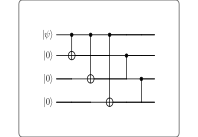
\includegraphics[width=0.7\textwidth]{../../images/steane_code_circuit.svg}
\end{center}

\subsection{数学推导}

Steane 码基于经典 Hamming 码 $[7,4,3]$：
\begin{equation}
|0\rangle_L = \frac{1}{\sqrt{8}} \sum_{x \in C} |x\rangle
\end{equation}
\begin{equation}
|1\rangle_L = \frac{1}{\sqrt{8}} \sum_{x \in C} |x \oplus 1111111\rangle
\end{equation}

其中 $C$ 是 Hamming 码的码字集合。

\textbf{校验矩阵}：
\begin{equation}
H = \begin{pmatrix} 0 & 0 & 0 & 1 & 1 & 1 & 1 \\ 0 & 1 & 1 & 0 & 0 & 1 & 1 \\ 1 & 0 & 1 & 0 & 1 & 0 & 1 \end{pmatrix}
\end{equation}

\subsection{几何解释}

Steane 码利用 Hamming 码的校验结构，通过测量校验子来检测和纠正错误。

\section{代码详解}

\begin{lstlisting}[style=python]
from quonic.qec import steane_code

# steane_code(error_type, error_qubit)
# error_type: "X", "Z", or "Y"
# error_qubit: which qubit has the error
result = steane_code(error_type="X", error_qubit=0)

# result.original: original state
# result.corrected: corrected state
print(f"Corrected: {result.corrected}")
\end{lstlisting}

\section{进阶用法}

\subsection{场景 1：不同错误类型}

\begin{lstlisting}[style=python]
for error_type in ["X", "Z", "Y"]:
    result = steane_code(error_type=error_type, error_qubit=0)
    print(f"{error_type} error: {result.corrected}")
\end{lstlisting}

\section{适用场景}

\subsection{量子计算}

Steane 码是高效的量子纠错码。

\subsection{量子通信}

Steane 码可以保护量子通信中的量子态。

\section{常见问题}

\subsection{Steane 码需要多少量子比特？}

需要 7 个物理量子比特编码 1 个逻辑量子比特。

\subsection{Steane 码和 Shor 码有什么区别？}

Steane 码用 7 个量子比特，Shor 码用 9 个。Steane 码效率更高。

\section{学习路径}

\subsection{前置知识}
\b\begin{itemize}
  \item Shor 码
  \item Hamming 码
  \item 量子测量
\end{itemize}

\subsection{继续学习}
\b\begin{itemize}
  \item 表面码
  \item 颜色码
  \item 拓扑纠错
\end{itemize}

\section{完整示例代码}

\subsection{示例 1：基本 Steane 码}

\begin{lstlisting}[style=python]
from quonic.qec import steane_code

result = steane_code(error_type="X", error_qubit=0)
print(f"Corrected: {result.corrected}")
\end{lstlisting}


\section{下载}

\begin{itemize}
  \item [steane_code.py](https://github.com/ChrisLee0721/QuoNic/blob/main/examples/steane_code/steane_code.py)
\end{itemize}

\end{document}
